\documentclass[10pt,letterpaper]{article}
\usepackage{tikz,amsmath,amssymb,geometry,graphicx}
\usepackage{enumitem}
\usetikzlibrary{shapes.geometric}
%\settextfont{B Nazanin}
\usepackage{lipsum}
\setlength{\parskip}{3mm}
\setlength{\parindent}{0mm}
\begin{document}
\Large
\begin{center}
In the name of beauty

1st problem set of ComNet course

\hrulefill
\end{center}
Q1)

Determine the following statements as true or false with enough reasons.
\begin{enumerate}[label=\alph*-]
\item
Transmission delay is defined as the time elapsed when a single bit physically traverses a link.
\item
Packet Switching is practically more complicated than Circuit Switching while being more suitable to real-time applications.
\item
In a host-to-host transmission, packets only traverse a collection of links in the network.
\item
With traffic intensity being close to 1, the queuing delay of the packets tends to zero.
\item
Link-layer switches are typically capable of processing the packets up to the layer 3.
\item
SMTP and FTP are examples of layer 1 protocols while TCP is a transport layer protocol.
%\item
%API is a set of rules 
%\item
%For economical reasons, exploiting optical fibers is not recommended in long-haul network
\end{enumerate}
Q2)

What is the difference between \textbf{Virus} and \textbf{Worm}?

Q3)

Consider the following network in which node A wants to send packets to node B through a router and two links:
\begin{figure}[ht]
\Large
\centering
\includegraphics[width=140mm]{p2p}
%\begin{tikzpicture}
%\node[draw=blue,circle,line width=2] (A) at(0,0) {A};
%\node[draw=blue,circle,line width=2] (B) at(12,0) {B};
%\node[ellipse, draw=blue,line width=2] (R) at (0,0) {};
%\end{tikzpicture}
\end{figure}
Assume the transmission rate of the links 1 and 2 to be 100Mbits/sec and 50Mbits/sec, respectively and both of the links be 10km long. The speed of light is $2\times 10^8$m/s in the links.
\begin{enumerate}[label=\alph*-]
\item
What is the end-to-end propagation delay?
\item
Assume node A wishes to transmit 4 consecutive, 12.5Kbytes packets, each of which being sent at a single 1ms time slot, that is, packet 1 is sent in the first time slot, packet 2 is sent in the second time slot and so on. If the router does not impose processing delay on packets, how much buffer capacity would it need for storing incoming packets in the 4th time slot due to the queuing delay of the previously received packets?
\item
Is there any bottleneck link and if so, which one and why?
\end{enumerate}

Q4) In the following network topology, each link is vulnerable to be brought down with a probability of $p$ independent of the other ones. What is the probability that there exists a path between nodes A and H with a throughput of $2R$? (The total throughput of a path is defined as the maximum rate at which bits can be sent over the path)
\begin{figure}[ht]
\centering
\includegraphics[width=140mm]{Q5}
\end{figure}

Q5)

In the following network sketch, node A can send packets arbitrarily over each of the three paths to routers R1, R2 and R3 and node B can receive packets arbitrarily too. If each link fails to transmit data with a probability of $p$ independent of the other ones.
\begin{figure}[ht]
\centering
\includegraphics[width=140mm]{p2p_multi}
\end{figure}
\begin{enumerate}[label=\alph*-]
\item
What is the probability that a packet initiated at node A, finally reaches its destination at node B?
\item
If each link has a throughput of $R$, what would be the effective throughput between nodes A and B? (i.e. the throughput that node A actually exploits and senses in transmission to node B; you need to do some probability calculations to obtain the answer!)
\end{enumerate}
%\noindent
%سوال 1) درستی یا نادرستی گزاره های زیر را با بیان دلایل کافی تحقیق کنید.
%
%1. برای شدت ترافیک نزدیک به $1$، تاخیر صف
%\footnote{
%\lr{Queuing delay}
%}
% بسته ها به سمت صفر میل می کند.
%
%2. داده برای انتقال از یک هاست
%\footnote{
%\lr{Host}
%}
% به هاست دیگر، فقط از مجموعه ای از لینک ها می گذرد.
%
%3. \lr{API} 
%مجموعه‌ی قوانینی است که برنامه‌ی سمت فرستنده باید پیروی کند تا اینترنت قادر به انتقال داده به برنامه‌ی مقصد باشد.
%
%4. \lr{Packet Switching}
% پیاده سازی پیچیده تر و پر هزینه تری نسبت به \lr{Circuit Switching} ایجاب می کند؛ ولی در مقابل برای کاربردهای بلادرنگ
%\footnote{
%\lr{Real-time}
%}
% مناسب تر است.
%
%5. یک پروتکل، فرمت و ترتیب پیامهای جابجاشده بین دو واحد مخابراتی را مشخص می کند و به اعمال انجام شده در ارسال و یا دریافت پیام نظارتی ندارد.
%
%6. در سمت کاربر، \lr{DSLAM} وظیفه ی جداسازی سیگنال های تلفنی و دیتای اینترنتی را در \lr{cable Internet access} بر عهده دارد.
%
%7. در معماری \lr{PON} همه ی بسته های ارسال شده از \lr{OLT} به سمت \lr{Splitter}، در \lr{Splitter} تکثیر می شوند.
%
%8. به دلایل اقتصادی، از فیبر نوری نمی توان در شبکه های \lr{long-haul} استفاده کرد.
%
%9. لایه‌ی پروتکل فقط در نرم افزار پیاده سازی می‌شود.
%
%10. تنها یک پروتکل \lr{IP} وجود دارد و تمام اجزای اینترنت که یک لایه‌ی شبکه دارند، باید از این پروتکل تبعیت کنند.
%
%\noindent
%سوال 2) تفاوت ویروس (\lr{Virus}) و کرم (\lr{Worm}) چیست؟
%
%\noindent
% سوال 3) در یک روتر، بسته
%\footnote{
%\lr{Packet}
%}
% هایی با طول 8 بیت به ورودی آن ارسال می شوند و نرخ دریافت بسته ها در ورودی از توزیع زیر پیروی می کند:
%\eqn{
%f_A(a)={(3.35)^a\cdot e^{-3.35}\over a!}
%}{}
%نرخ خروجی بیت در روتر نیز دارای توزیع زیر است:
%\eqn{
%R\sim \mathcal{U}(35,40)
%}{}
%\indent
%الف) متوسط شدت ترافیک
%\footnote{
%\lr{Traffic Intensity}
%}
% را در این روتر محاسبه کنید.
%
%\indent
%ب) اگر چهار بسته به صورت پشت سر هم وارد این روتر شوند، متوسط تاخیر ارسال
%\footnote{
%\lr{Transmission delay}
%}
% بسته‌ی چهارم چه 
%\indent
%میزان خواهد بود؟ (تاخیر ارسال بسته‌ی اول را صفر در نظر بگیرید)
%\noindent
%سوال 4) در شبکه ی زیر، اگر احتمال خرابی هر لینک مستقل از سایرین برابر $p$ باشد، احتمال صحت کل مسیر را از $A$ تا $B$ به دست آورید.
%\begin{center}
%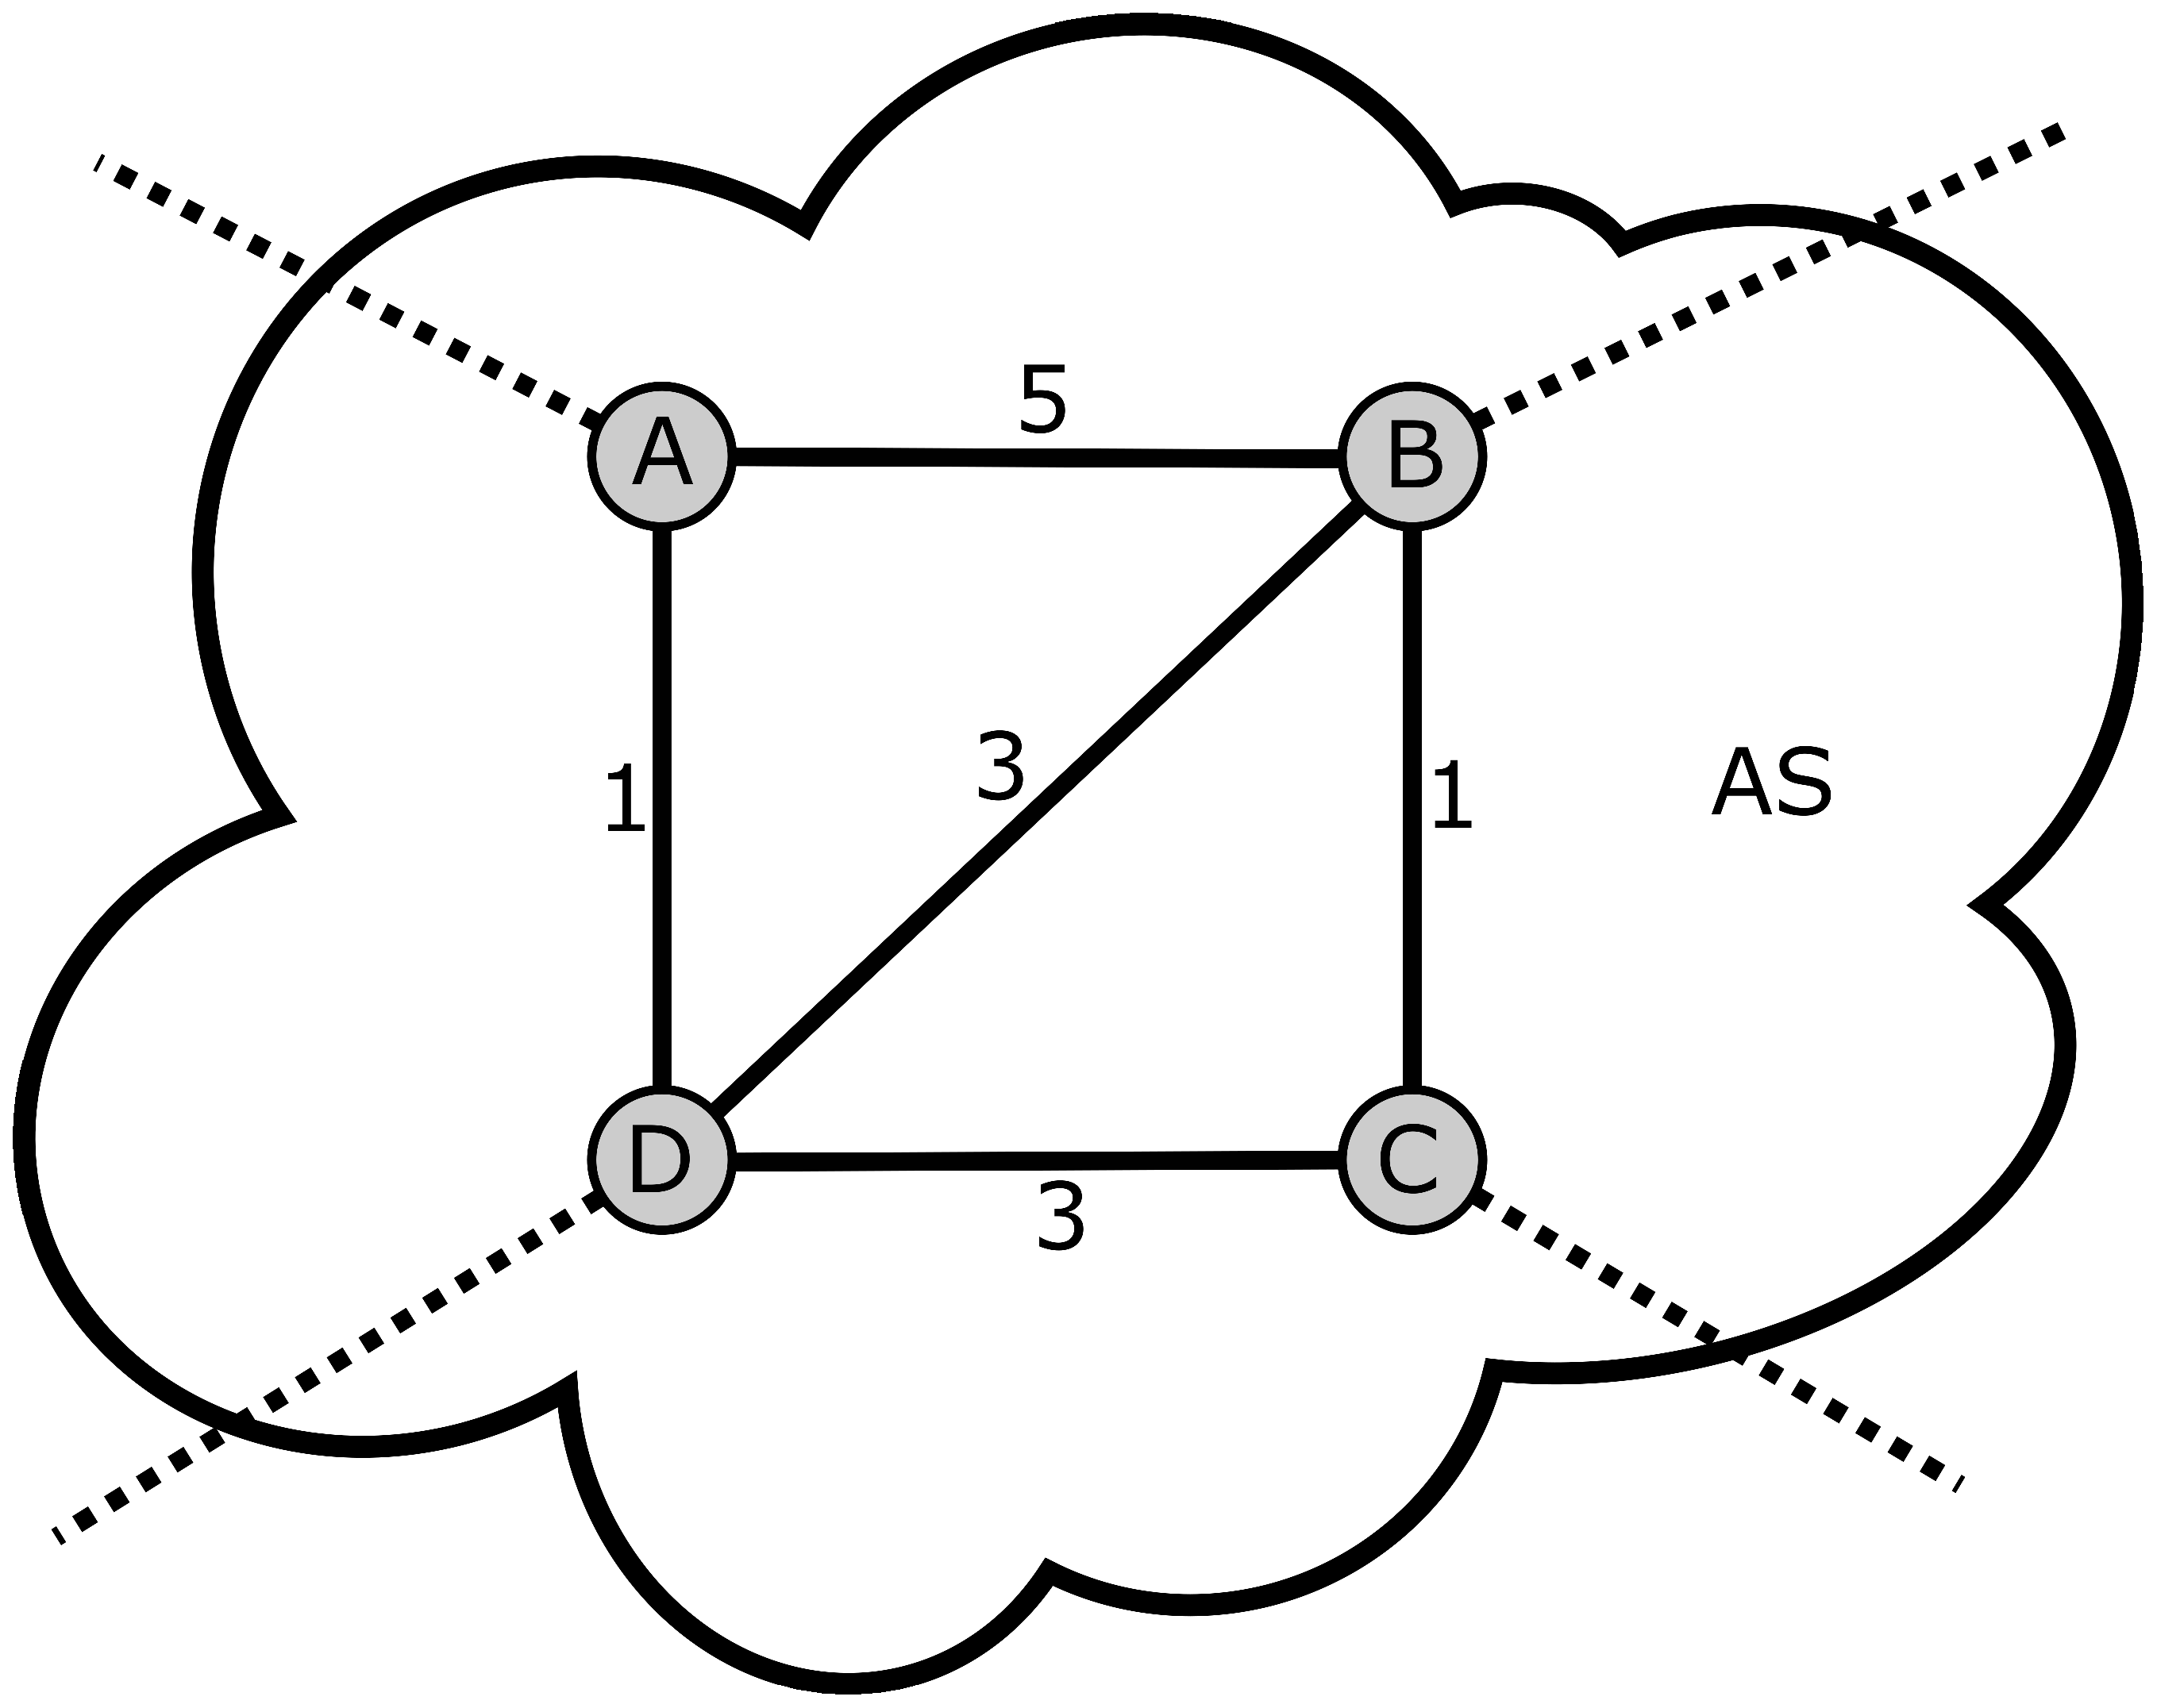
\includegraphics[width=100mm]{Q4}
%\end{center}
%سوال 5) در شبکه ای با توپولوژی زیر، در چه صورت و با کدام احتمال حداکثر \lr{throughput} برای مسیر $A-H$ برابر $2R$ می باشد؟ (احتمال خرابی هر لینک مستقل از سایرین برابر $p$ می باشد)
%\begin{center}
%\includegraphics[width=100mm]{Q5}
%\end{center}
%\noindent
%سوال 6) در شبکه‌ی زیر، فرض کنید نرخ ورود بیت به روتر برابر 
%$1\text{\lr{Mbps}}$
%، حجم هر بسته برابر 
%$1\text{\lr{kbytes}}$
%، تاخیر پردازش هر بسته برابر 
%$12\text{\lr{msec}}$
%، طول لینک برابر 200 متر و سرعت انتشار در لینک برابر 
%$2\times 10^8 \text{\lr{m/s}}$
% است. همچنین  نرخ خروج بیت از روتر را بینهایت بگیرید.
%
%الف) تاخیر ارسال را برای بسته‌ی دهم محاسبه کنید.
%
%ب) تاخیر کلی ای را که بسته‌ی دوم در ارسال از \lr{A} به \lr{B} تجربه می کند محاسبه کنید.
%
%ج) به مدت چند میلی ثانیه و برای اولین بار، حجم اشغال شده‌ی بافر برابر 
%$2\text{\lr{kbytes}}$
% خواهد بود؟ (حالتی که یک بسته بلافاصله وارد بافر می‌شود و تنها بسته‌ی کنونی بافر بلافاصله از آن خارج می‌شود، $1\text{\lr{kbytes}}$ از حجم بافر را اشغال می‌کند. به عبارت دیگر باید مدت زمان غیرصفری محاسبه شود که دو بسته همزمان در بافر حضور داشته باشند)
%\begin{center}
%\includegraphics[width=100mm]{Q6.jpg}
%\end{center}
\end{document}